\documentclass[a4paper,10pt]{article}


\usepackage[utf8]{inputenc}
%\usepackage{mathtools}
\usepackage{graphicx}
\graphicspath{{img/}}
\usepackage[italian]{babel}
\usepackage{float}
\usepackage{amsmath}
\usepackage{verbatim}
\usepackage{siunitx}

\title{Analisi ponte trifase total-controllato}
\author{Olivieri Daniele}
\date{18 novembre 2019}

\pdfinfo{%
  /Title    (Analisi ponte trifase total-controllato)
  /Author   (Olivieri Daniele)
  /Creator  (Olivieri Daniele)
  /Producer ()
  /Subject  (Elettronica di Potenza)
  /Keywords (FEP, Power Electronics, Three Phase Converter)
}

\begin{document}
\maketitle

\begin{abstract}
 ciao ciao
\end{abstract}

\begin{comment}
\section{Introduzione} %C'è l'abstract come introduzione(?)
Elenco canali oscilloscopio:
1 - Giallo: Vl sul carico
2 - Verde: Vr sulla resistenza o corrente nel carico
3 - Blu: corrente al secondario
4 - Rosso: corrente al primario

Trasformatore stella con neutro al primario - stella al secondario
Riferimenti degli impulsi sulla concatenata
V1/V2 = 9.524
Tensione ingresso 220 V starred
\end{comment}


\section{Norme tecniche che disciplinano la procedura di prova}
Il comitato tecnico che disciplina l'elettronica di potenza è il CT 22 e la norma
di riferimento per la prova è la CEI EN 60146: ``Convertitori a semiconduttore''.

\section{Strumenti utilizzati}
Per effettuare la prova sono stati utilizzati i seguenti strumenti di misura:
\begin{itemize}
 \item Oscilloscopio a 4 canali Keysight DSO-X 2014A;
 \item Trasduttore di corrente a 2 canali ad effetto Hall da 5 A, artigianale.
\end{itemize}

\section{Componenti utilizzati}
I componenti sottoposti a prova sono sei tiristori \%INSERISCI MODELLO\%.
L'alimentazione del ponte è fornita tramite un trasformatore trifase TTSK0.20 da 
200 VA conforme alla norma di sicurezza CEI 96-7.
Si può approssimare il rapporto tra le due tensioni nominali del trasformatore uguale al 
rapporto di trasformazione pari quindi a 9.524.

Il trasformatore è collegato a stella con neutro alla rete trifase con una tensione
concatenata di $\SI{220}{\volt_{RMS}}$ mentre il secondario è collegato a stella 
senza neutro alle tre gambe del ponte.

Il carico è composto da un induttore da $\SI{100}{\milli\henry}$ e
un resistore in serie da $\SI{10}{\ohm}$.



\section{Schema elettrico del circuito di prova}
Il seguente schema rappresenta la struttura in esame con le relative sonde
di misura.

I trasduttori di corrente sono stati rappresentati con degli
amperometri. Il voltmetro collegato al canale 1 permette di visualizzare la 
tensione sul carico, il voltmetro collegato al canale 2, tramite una costante di 
attenuazione di valore pari alla resistenza, permette di misurare 
la corrente che circola nel carico.


\begin{figure}[H]
 \centering
 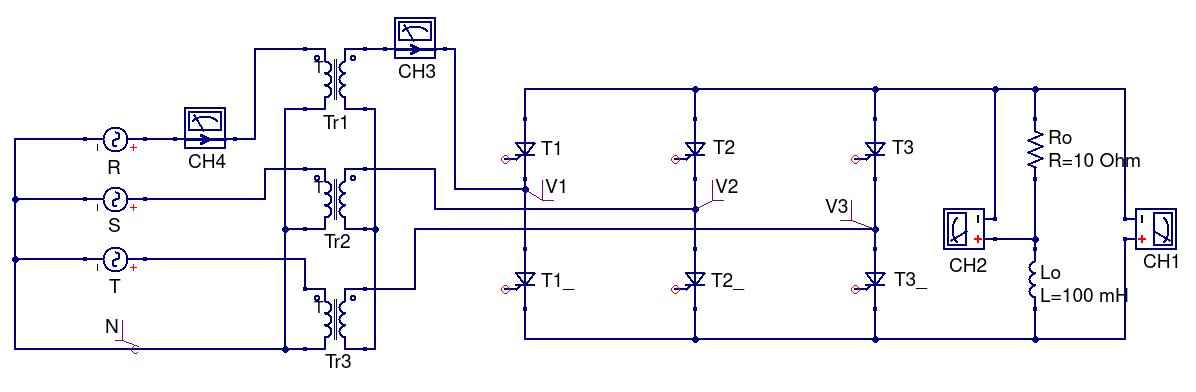
\includegraphics[keepaspectratio=true,width=1\linewidth]{circuito_qucs.png}
 % circuito_qucs.png: 1193x395 px, 115dpi, 26.35x8.72 cm, bb=0 0 747 247
 \caption{Struttura e circuito di misura}
 \label{fig:circuito}
\end{figure}

Un unico gate driver trifase appositamente realizzato gestisce il turn-on
dei singoli tiristori.

Il trasformatore trifase è a flusso vincolato poichè sono presenti 
solo tre colonne, questa proprietà non è individuabile dallo schema in cui 
è presente un banco trimonofase a flusso libero.

In seguito si riporta una foto del banco di prova:
\begin{figure}[H]
 \centering
 \includegraphics[keepaspectratio=true,width=1\linewidth]{circuito_reale.png}
 \caption{Circuito realizzato per la misura}
 \label{fig:circuito_reale}
\end{figure}

\section{Richiami teorici}
La rete trifase fornisce una terna di tensioni sinusoidali ad una frequenza di
$\SI{50}{\hertz}$ sfasate tra loro con un angolo di \ang{120}
così rappresentabile:

 \begin{figure}[H]
 \centering
 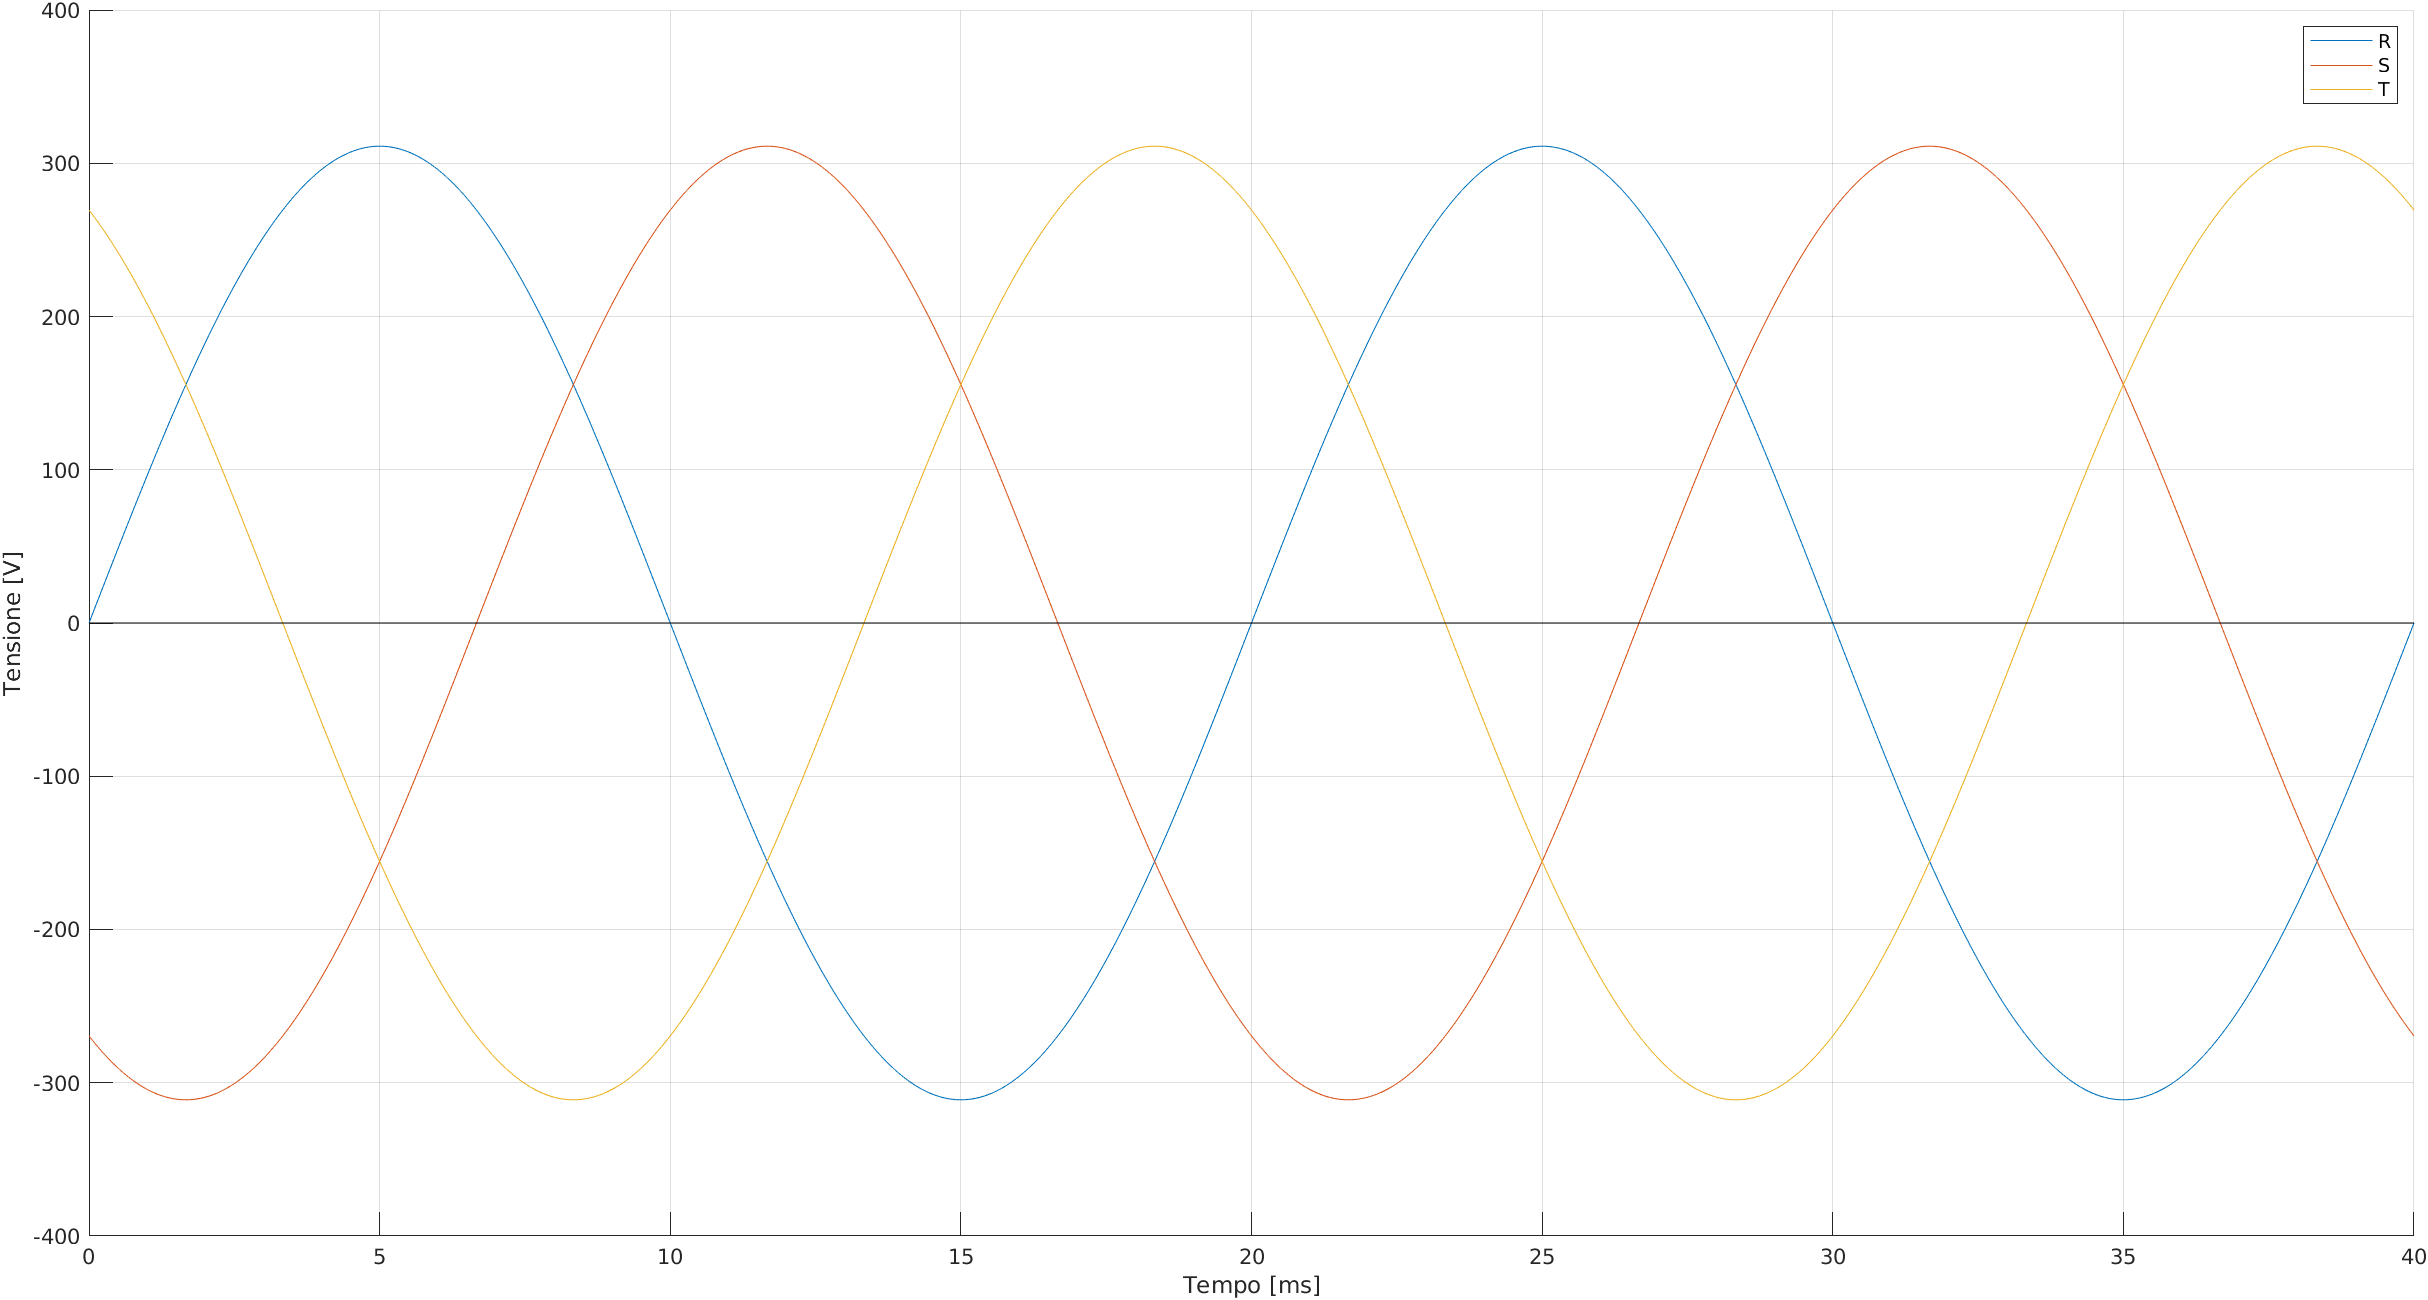
\includegraphics[keepaspectratio=true,width=0.95\linewidth]
 {sinusoidi_trifase.png}
 % circuito_qucs.png: 1193x395 px, 115dpi, 26.35x8.72 cm, bb=0 0 747 247
 \caption{Terna trifase}
 \label{fig:terna_trifase}
\end{figure}

Per il turn-on di un tiristore è necessario che si verifichino le seguenti
condizioni:
\begin{itemize}
 \item \(\exists\) una maglia di corrente possibile che coinvolga il componente;
 \item \(V_{AK} \geq 0\) la tensione anodo-catodo sia maggiore di 0;
 \item \(I_G \geq I_{GT}\) la corrente di gate sia maggiore di 
 un certo valore di soglia (trigger).
\end{itemize}
È possibile dividere i tiristori in due gruppi, superiore ed inferiore. 

Quelli del gruppo superiore \((T1,T2,T3)\) hanno gli anodi collegati tra loro
e con il carico. Ai catodi invece, sono collegate le tre fasi e i tiristori 
vedono le rispettive tensioni stellate riferite rispetto al centro stella formatosi al secondario del trasformatore.

Per quanto riguarda i tiristori del gruppo inferiore \((T1\_,T2\_,T3\_)\) invece
si presenta la situazione opposta, i catodi sono in comune tra essi e con il carico,
gli anodi sono connessi all'alimentazione e quindi ai catodi dei tiristori del gruppo precedente.

Trascurando la caduta di tensione sui tiristori si può assumere che, tramite un
opportuno driving dei componenti, si può fornire al carico la tensione
concatenata tra due fasi opportunamente scelte.
è possibile rappresentare le tensioni concatenate in un periodo di tempo nel seguente modo:
 \begin{figure}[H]
 \centering
 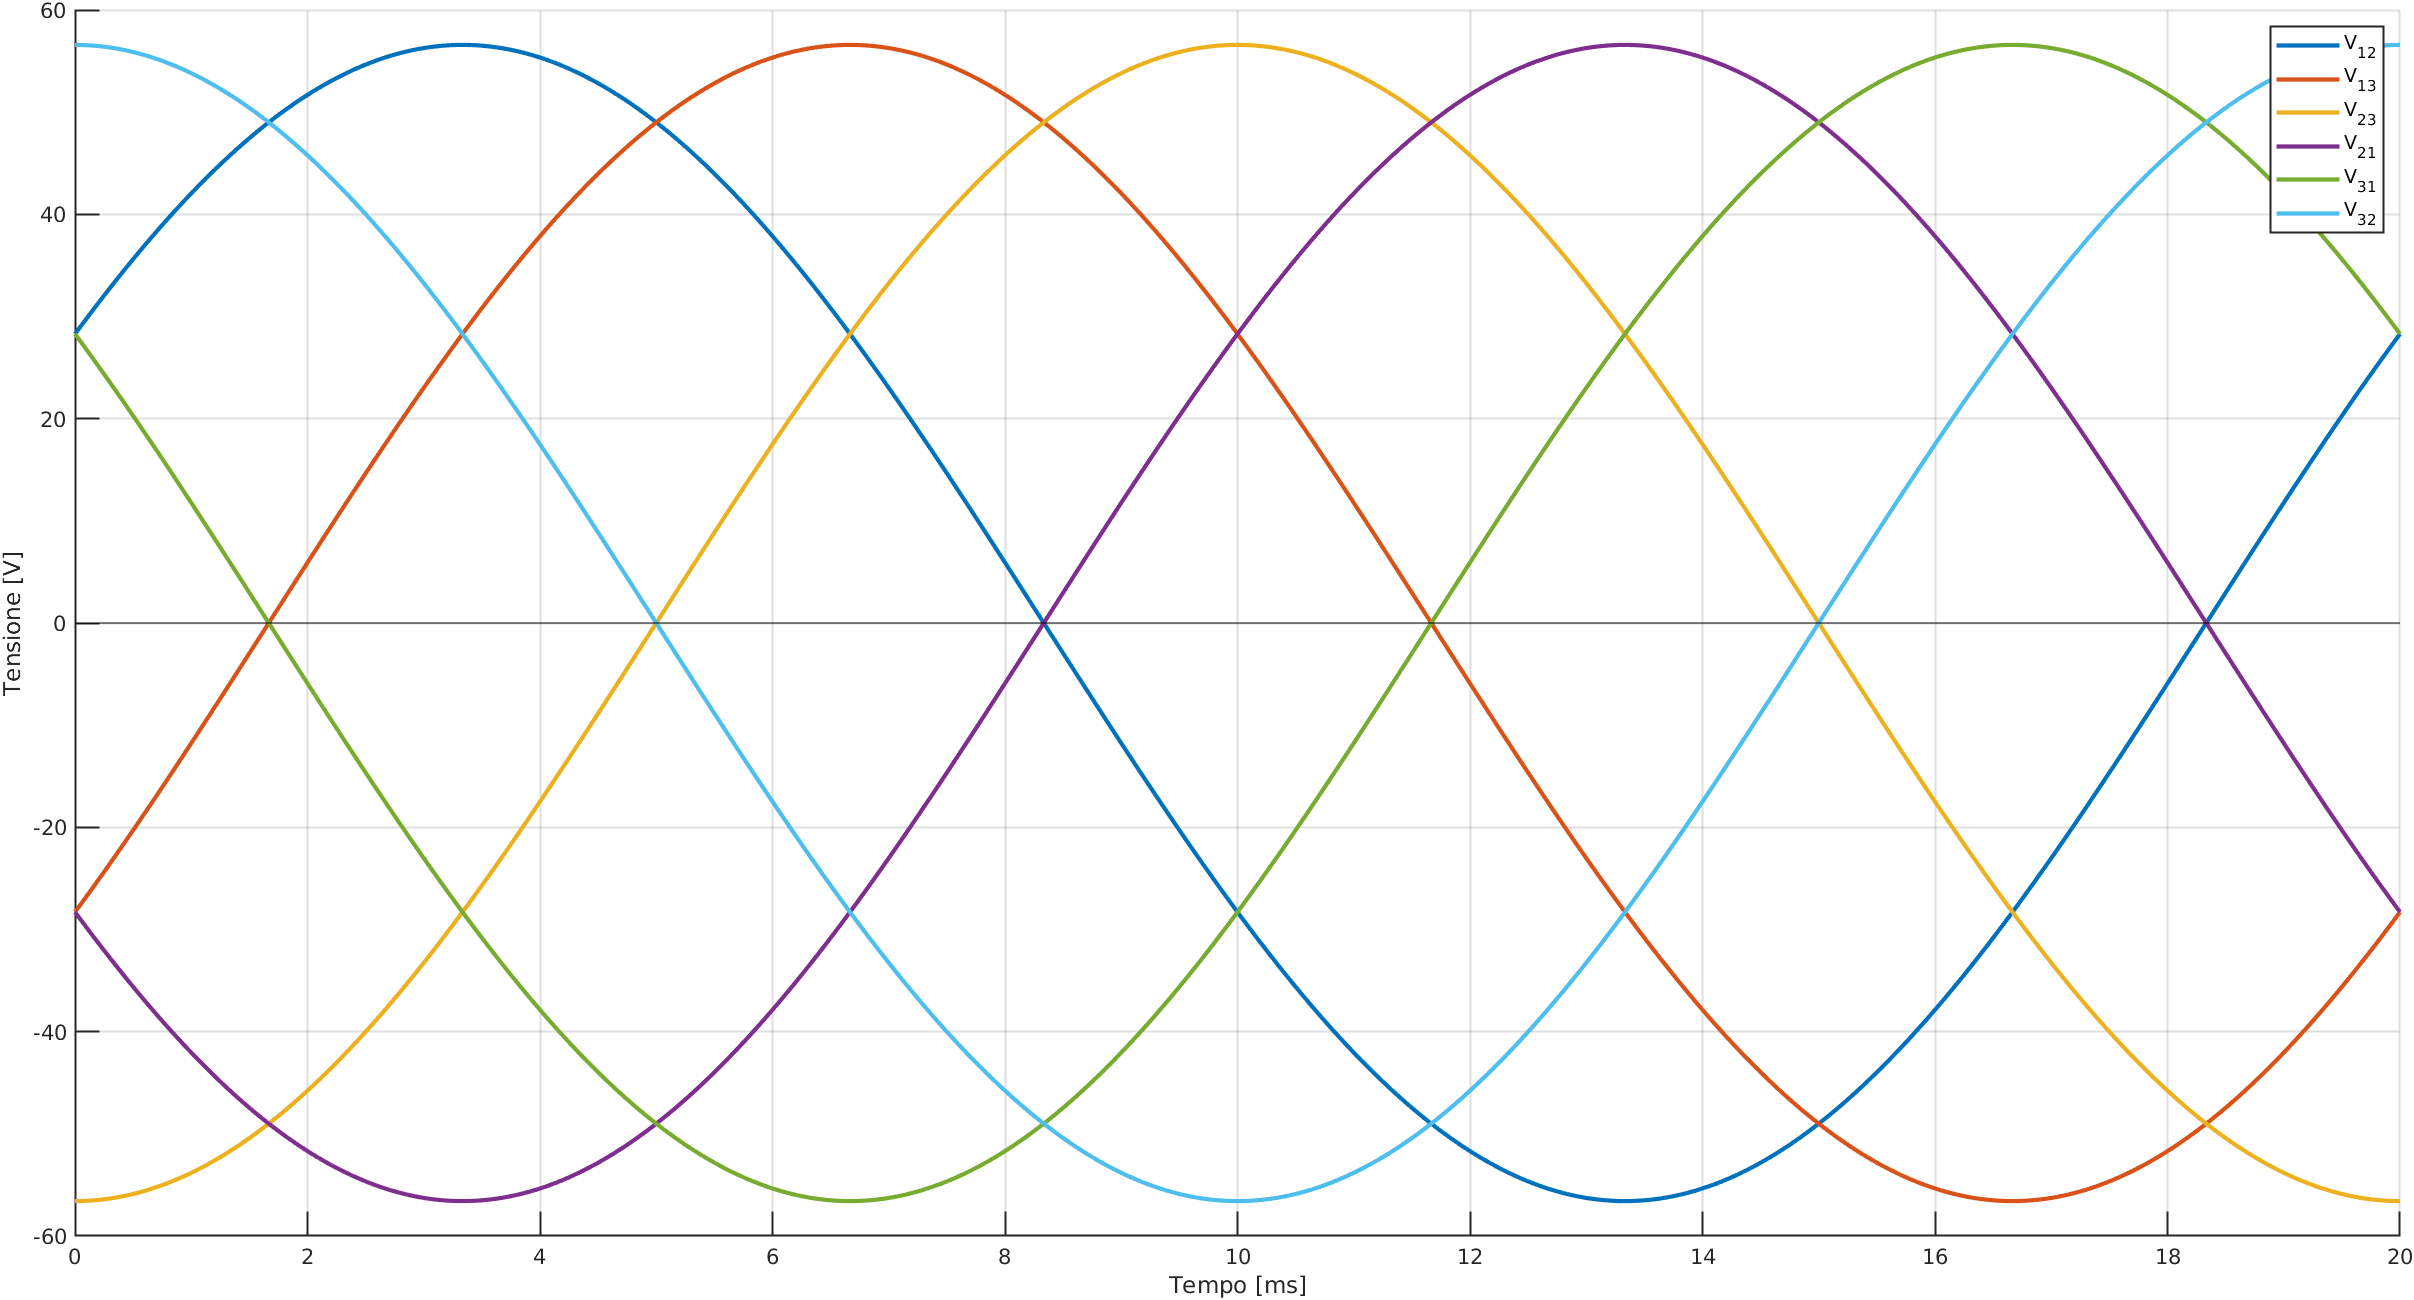
\includegraphics[keepaspectratio=true,width=0.95\linewidth]
 {concatenate_carico.png}
 \caption{Andamento delle tensioni concatenate a valle del trasformatore}
 \label{fig:concatenate}
\end{figure}

Osservando l'immagine si suppone che inizialmente conducano i tiristori \(T3\_\) e \(T2\),
dopo un tempo pari a \(\frac{1}{6}\cdot \frac{T}{2}\) ovvero 
$\SI{1.667}{\milli\second}$ la tensione \(V_{12}\) sarà maggiore 
di \(V_{32}\); impulsando quindi il tiristore \(T1\_\) esso andrà in conduzione perchè, tramite la precedente conduzione di \(T3\_\), il potenziale al suo catodo sarà V3 e quindi la tensione anodo-catodo sarà pari a \(V_{13} > 0 \).
In prima approssimazione è possibile considerare il tempo di commutazione nullo;
la conduzione di \(T1\_\) porta il potenziale V1 al catodo di \(T3\_\) e 
quindi la tensione \(V_{31} < 0\) ai suoi capi, ne consegue quindi
l'interdizione di \(T3\_\).
La conduzione di \(T1\_\) e \(T2\) porta sul carico la tensione \(V_{12}\).
\smallskip

Queste considerazioni si possono ripetere per le commutazioni successive, ipotizzando
di impulsare i componenti quando due tensioni concatenate passano per lo zero si può 
ottenere la seguente tabella:

\begin{center}
\begin{tabular}{c|c|c}
  Tempo [$\SI{}{\milli\second}$]&Tiristore impulsato&Tensione sul carico\\ \hline
  10/6 & \(T1\_\) & \(V_{12}\) \\
  5    & \(T3\)   & \(V_{13}\) \\
  25/3 & \(T2\_\) & \(V_{23}\) \\
  35/3 & \(T1\)   & \(V_{21}\) \\
  15   & \(T3\_\) & \(V_{31}\) \\
  55/3 & \(T2\)   & \(V_{32}\)
\end{tabular}
\end{center}


Poichè la frequenza di alimentazione può non essere necessariamente pari a 
$\SI{50}{\hertz}$, è comodo rappresentare le tensioni in un dominio angolare anzichè 
temporale, si fissa ovvero il periodo di tempo \(T\) pari ad un angolo giro ossia 
\(2\pi\); il rapporto tra l'angolo giro e il periodo di una forma d'onda prende il
nome di pulsazione \(\omega\) e si misura in $\SI{}{\radian\per\second}$.
\smallskip

Nonostante il tiristore sia un componente controllabile solo nel turn-on, questa 
struttura permette la commutazione forzata dal turn-on di un secondo tiristore,
per questo motivo si classifica come struttura total-controllata.
È possibile infatti ritardare il comando d'impulso di un certo angolo \(\alpha\) in
modo tale da modificare la forma d'onda di tensione sul carico e soprattutto il suo valore medio.

Sia \(\alpha\) l'angolo d'impulso dei componenti, riferito rispetto al valore nullo
delle tensioni concatenate, è possibile calcolare il valore medio della tensione in uscita.
Usando la definizione di media integrale per le funzioni periodiche:

\begin{equation}
 V_0 \stackrel{def}{=} \frac{1}{T}\int_T v_0(t) dt
 \label{eq:def_media_integrale}
\end{equation}
Traslando l'intervallo di analisi in ritardo di un angolo pari a \(\frac{\pi}{6}\) 
è possibile notare che le forme d'onda consecutive sono tutte identiche fra loro e pari %metti qua le coppolette se ci riesci
a 6 in un periodo, sfruttando questa proprietà si può calcolare l'integrale per una forma d'onda e poi moltiplicarlo per 6.
La forma d'onda da integrare è quindi la cuspide di un coseno, il valore medio di 
tensione in uscita si calcola quindi nel seguente modo:
\begin{equation}
 V_0 = \frac{6}{2\pi} \int_{-\frac{\pi}{6}+\alpha}^{\frac{\pi}{6}+\alpha}
 V\cdot \cos (\omega t)\ d\omega t
 %\label{eq:}
\end{equation}
dove \(V\) è il valore di picco della tensione concatenata al secondario del trasformatore
pari a \(N\cdot\sqrt2\sqrt3\cdot V_{IN_{RMS}} \) con \(N\) pari al rapporto di trasformazione
e \(V_{IN_{RMS}} \) il valore efficace della tensione in ingresso (stellata).
Ignorando il rapporto di trasformazione ci si riferirà per semplcità con \(V_{IN}\)
alla tensione al secondario del trasformatore.
%svolgi due conti, lo faccio più tardi mi scoccio

\begin{equation}
 V_0 = \frac{3}{\pi} \sqrt{2} \sqrt{3} V_\lambda \cos\alpha
 \label{eq:valore_medio_tensione_ponte}
\end{equation}


\section{Descrizione della prova eseguita}
%Inserisci immagini circuito reale
La prova è stata eseguita in un primo momento su un carico puramente resistivo, 
è possibile vedere in seguito le forme d'onda di tensione e corrente, simili a quelle 
descritte analiticamente:
\begin{figure}
 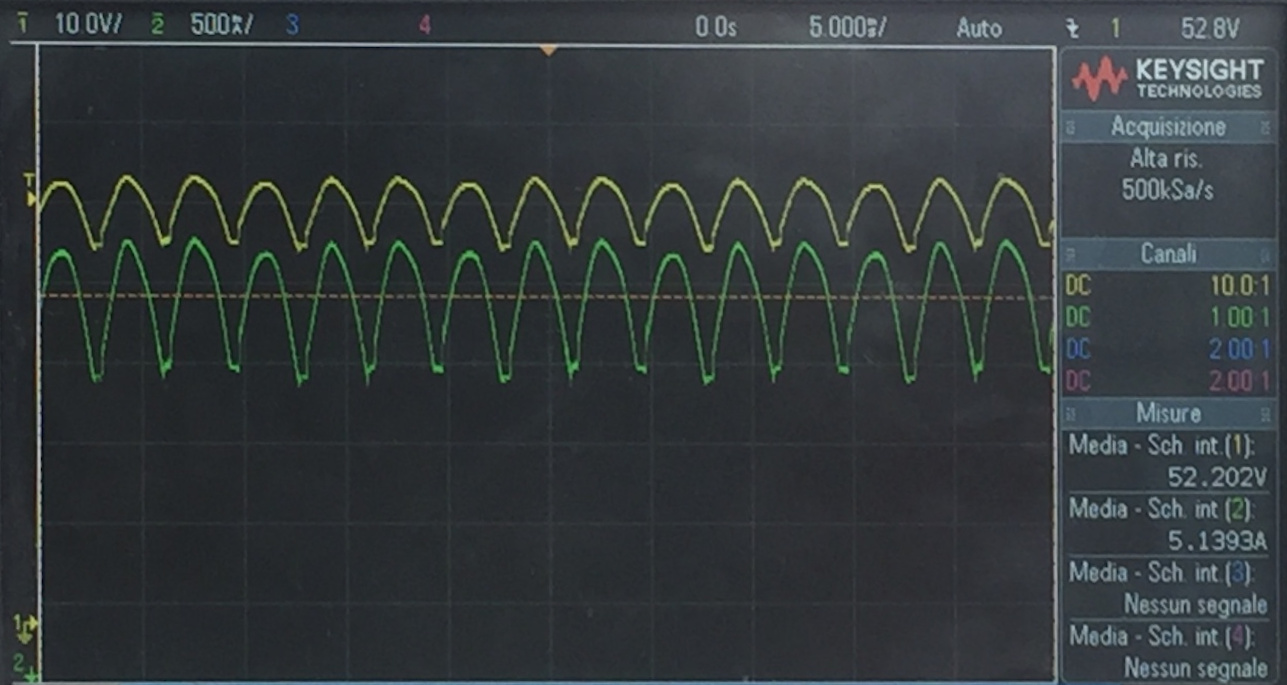
\includegraphics[keepaspectratio=true,width=0.9\linewidth]
 {tensione_e_corrente_2.jpg}
 \caption{Giallo: \(V_0\) \quad Verde: \(I_0\)}
 \label{fig:tensioni_carico_R}
\end{figure}


\section{Risultati ottenuti}
%In questa sezione inserisci le immagini dell'oscilloscopio


\end{document}
